\noindent\fbox{\begin{minipage}{\dimexpr\textwidth-2\fboxsep-2\fboxrule\relax}
\vspace{3 mm}
 What is an $n$ dimensional hypercube? 
\begin{enumerate}[label= ]
\item \textbf{Bit definition}: Two vertices $x$ and $y$ are adjacent
and only if $x$ and $y$ differ in exactly one bit 
position. 
\item \textbf{Recursive definition}: Define the 0-subcube as the $(n-1)$ 
dimensional hypercube with vertices labeled 0x (x is an element 
of $(0, 1)^{n-1}$). Do the same for the 1-subcube with vertices labeled 1x. Then an 
$n$ dimensional hypercube is created by placing an edge between 
0x and 1x in the 0-subcube and 
1-subcube respectively.
\end{enumerate}
\end{minipage}}

\begin{figure}[h]
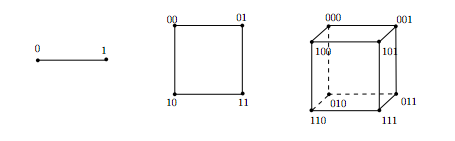
\includegraphics{hypercube}
\centering
\end{figure}

